\documentclass[qo.tex]{subfiles}

\begin{document}
\part{Quantum Theory In Condensed Matter}
\chapter{Bose-Einstein Statistics}
\section{Statistical Ensembles}
In statistical mechanics, one frequently formally considers $N$ copies of the system under consideration. 
Such an assembly is a \emph{statistical ensemble.}
\begin{itemize}
    \item In the \emph{microcanonical ensemble}, each copy has the same total poarticle number $N$ and total energy $U$.
    \item In the \emph{canonical ensemble}, each copy has the same total particle number $N$, however the total energy may fluctuate. 
        The system is considered to be in equilibrium with an external heat bath (maintaining a constant temperature $T$.
    \item In the \emph{grand canonical ensemble}, the total particle number and the total energy may fluctuate. 
        The system is considered to be in equilibrium with an external heat bath, and a particle bath (maintaining a constant chemical potential $\mu$).
\end{itemize}
We are generally interested in macroscopic systems of an effectively infinite number of particles, and may take the \emph{thermodynamic limit} $V\to\infty$ in which the particle density $n=N/V$ is held constant. 
The thermodynamic predictions of the three ensembles are then identical, and it is usually more convenient to use the grand canonical ensemble. 
If the $N$-body quantum states of $N$ quantum particles have energy $E_n^{(N)}$ for $n=1,2,\dots$, then in the grand canonical ensemble, each state occurs with probability
\begin{align}
    P_n^{(N)} &= \frac{1}{Z}\exp\left(-\frac{1}{k_BT}\left[E_n^{(N)}-\mu N\right]\right),
    \text{ where } Z = \sum_{N,k} \exp\left(-\frac{1}{k_BT}\left[E_n^{(N)}-\mu N\right]\right)
\end{align}
is the \emph{grand partition function.}

\section{Particle with Periodic Boundary Conditions}
Consider a point particle of mass $m$ moving within a volume $V=L_xL_yL_z$, where $L_i$ are lengths in the $i=x,y,z$ directions. 
The Hamiltonian 
\begin{equation}
    \hat{H} = \frac{1}{2m}\left(\hat{p}_x^2+\hat{p}_y^2+\hat{p}_z^2\right),
\end{equation}
and the eigenstates of the momentum operator $\hat{p}=(\hat{p}_x,\hat{p}_y,\hat{p}_z)$ are also eigenstates of $\hat{H}$ (subject to periodic boundary conditions).
In the \emph{position representation}, they take the form of plane waves:
\begin{align}
    \psi_k(\vr) = \frac{1}{\sqrt{V}}e^{i\unl{k}\cdot\vr}, \text{ where } \unl{k} = \left(\frac{2\pi n_x}{L_x},\frac{2\pi n_y}{L_y},\frac{2\pi n_z}{L_z}\right).
\end{align}
The differences in $k$ between neighbouring eigenstates are $2\pi/L_i$, in the $i=x,y,z$ directions.
The $k$-space density of the available states is therefore
\begin{align}
    \rho(\unl{k}) = \frac{L_xL_yL_z}{(2\pi)^3} = \frac{V}{(2\pi)^3}.
\end{align}

\section{Spherical Shells in k}
We divide up $k$-space into thin concentric shells. 
A shell of radius $k_S$ and thickness $\delta k_S$ has volume $4\pi k_S^2\delta k_S$, and therefore contains $M_S$ states, where
\begin{align}
    M_S &= 4\pi k_S^2\delta k_S\rho(\unl{k}) = 4\pi k_S^2\delta k_S \frac{V}{(2\pi)^3}.
\end{align}
Each such quantum state has energy $\e_S=\hbar^2k_S^2/2m$, from which we can determine an energy increment $\delta\e_S=(\hbar^2/m)k_S\delta k_S$.
Hence, the number of available states between energies $\e_S$ and $\e_S+\delta\e_S$ is
\begin{align}
    M_S = Vg(\e_S)\delta\e_S, \text{ where } g(\e) = \frac{m^{3/2}}{\sqrt{2}\pi^2\hbar^3}\e^{1/2}
\end{align}
is the (energy) density of states per unit volume. 
\emph{All states on a given shell have the same energy.}

\section{Thermal Equilibrium and the Bose-Einstein Distribution}
Consider an \emph{ideal Bose gas}, i.e. a system of many identical, non-interacting bosons, e.g. in a box subject to periodic boundary conditions. 
In \emph{thermal equilibrium}, the particles are distributed so that the occupation numbers $N_S$ in each shell of energy $\e_S$ maximise the total entropy. 
This yields the \emph{Bose-Einstein distribution:}
\begin{align}
    f_{BE}(\e) = \frac{1}{e^{(\e-\mu)/k_BT}-1}.
\end{align}

\section{Particle Density in the Thermodynamic Limit}
Using the Bose-Einstein distribution in Eq (1.7), the total number of particles in a volume $V$ (subject to periodic boundary conditions) is
\begin{align}
    N &= \sum_{\unl{k}}\frac{1}{e^{(\e_{\unl{k}}-\mu)/k_BT}-1}.
\end{align}
Taking the thermodynamic limit $V\to\infty$, the possible $\unl{k}$ values tend to a continuum, and we replace the sum $\sum_{\unl{k}}$ with an integral $\int\rho(\unl{k})\,dk_x\,dk_y\,dk_z \equiv \int\rho(\unl{k})\,d^3k = [V/(2\pi)^3]\int\,d^3k$.
Hence
\begin{align}
    N &= \frac{V}{(2\pi)^3}\int \frac{d^3k}{e^{(\e_{\unl{k}}-\mu)/k_BT}-1} \implies n \equiv \frac{N}{V} = \frac{1}{(2\pi)^3}\int \frac{d^3k}{e^{(\e_{\unl{k}}-\mu)k_BT}-1}.
\end{align}
Recalling $V/(2\pi)^3\,d^3k = [V/(2\pi)^3]4\pi k^2\,dk = Vg(\e)\,d\e$, then in terms of the density of states per unit volume, $g(\e)$,
\begin{align}
    n = \int \frac{g(\e)\,d\e}{e^{(\e_{\unl{k}}-\mu)/k_BT}-1}.
\end{align}

\chapter{Bose-Einstein Condensation}
\section{Particle Density in Terms of the Fugacity}
Using the fugacity $z\equiv e^{\mu/k_BT}$ and $x\equiv \e/k_BT$, we can rewrite the particle density $n$ as
\begin{align}
    n &= \frac{(mk_BT)^{3/2}}{\sqrt{2}\pi^2\hbar^3}\ofnt \frac{ze^{-x}}{1-ze^{-x}}x^{1/2}\,dx.
\end{align}
Taylor expanding $(1-ze^{-x})^{-1}$ around $ze^{-x}=0$, we deduce the identity
\begin{align}
    ze^{-x}(1-ze^{-x})^{-1} &= ze^{-x}\left(1+ze^{-x}+z^2e^{-2x} + \dots\right) = \sum_{j=1}^\infty z^je^{-jx}.
\end{align}
As $x>0$, this expansion is convergent for $z<1$, and we can evaluate the integral over $x$ using:
\begin{align}
    \ofnt e^{-jx}x^{1/2}\,dx &= \frac{1}{j^{3/2}}\underbrace{\ofnt e^{-y}y^{1/2}\,dy}_{\equiv \Gamma(3/2)} = \frac{1}{j^{3/2}}\frac{\sqrt{\pi}}{2}.
\end{align}
This implies 
\begin{align}
    n &= \left(\frac{mk_BT}{2\pi\hbar^2}\right)^{3/2}g_{3/2}(z), \text{ where } g_{3/2}(z) = \sum_{j=1}^\infty \frac{z^j}{j^{3/2}}.
\end{align}
We therefore need to know something of the properties of $g_{3/2}(z)$ to evaluate the particle density $n$.

\section{Properties of g}
The series defining $g_{3/2}(z)$ converges when $|z|<1$, and diverges when $|z|>1$.
At $z=1$, it is just convergent:
\begin{align}
    g_{3/2}(1) &= \zeta(3/2) = 2.612, \text{ where } \zeta(s) \equiv \sum_{j=1}^\infty \frac{1}{j^s}
\end{align}
is the Riemann zeta function.
The derivative of $g_{3/2}(z)$, however, is infinite at $z=1$, since
\begin{align}
    \frac{d}{dz}g_{3/2}(z)\bigg|_{z=1} &= \frac{1}{z}\sum_{j=1}^\infty \frac{z^j}{j^{1/2}}\bigg|_{z=1} = \sum_{j=1}^\infty \frac{1}{j_{1/2}}
\end{align}
diverges.
With these limiting values, we can make a sketch of $g_{3/2}(z)$ for $0\leq z\leq1$:
\begin{figure}[H]
    \centering
    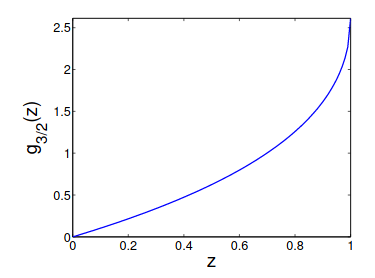
\includegraphics[scale=0.7]{g32.png}
\end{figure}

\section{Critical Temperature}
We can invert Eq (2.4) to get 
\begin{align}
    g_{3/2}(z) &= \left(\frac{2\pi\hbar^2}{mk_BT}\right)^{3/2}n.
\end{align}
If we are in a regime of high $T$ or low $n$, it follows that $g_{3/2}(z)$ must take a small value.
From the plot of $g_{3/2}(z)$ above, we see that this implies small $z$, which from the definition of $g_{3/2}(z)$ means we can approximate $g_{3/2}(z)\approx z$. 
Hence, recalling $z=e^{\mu/k_BT}$,
\begin{align}
    \mu &\approx -\frac32 k_BT\ln\left(\frac{mk_BT}{2\pi\hbar^2n^{2/3}}\right),
\end{align}
i.e., the chemical potential is negative. \\
As $n$ is fixed, it follows from Eq (2.4) that as $T$ is lowered (but assumed $T>0$), $z$ must increase, with maximum finite value of $z=1$, i.e. $\mu=0$.
It straightforwardly follows that this occurs at a \emph{critical temperature} (recalling $g_{3/2}(1)=2.612$) of 
\begin{align}
    T_C &= \frac{2\pi\hbar^2}{k_Bm}\left(\frac{n}{2.612}\right)^{2/3}.
\end{align}

\section{Macroscopic Occupation of the Ground State}
Recall that the Bose-Einstein distribution from Eq (1.7) predicts the occupation of $\e=\e_{\unl{k}=0}=0$ state to be 
\begin{align}
    N_0 &= \frac{1}{e^{-\mu/k_BT}-1}.
\end{align}
Hence, $\mu=0\implies N_0\to\infty$ (Bose-Einstein condensation).
Recalling that we are in the thermodynamic limit ($N,V\to\infty$), what this actually means is that $n_0=N_0/V$ is some finite fraction of $n$.
Rewriting Eq (2.10) for large $N_0$, we obtain 
\begin{align}
    \mu &= -k_BT\ln\left(1+\frac{1}{N_0}\right) \approx -\frac{k_BT}{N_0}.
\end{align}
Hence, as $N_0\to\infty$, $\mu\to0$.
Therefore, below $T_C$, the chemical potential $\mu$ is effectively 0.

\section{Below the Critical Temperature}
Below $T_C$, we must take $\vk=0$ point into account separately, and so we set $\mu=0$ and modify Eq (1.8) to
\begin{align}
    N &= N_0 + \sum_{\vk\neq0}^\infty \frac{1}{e^{\e_{\vk}/k_BT}-1}.
\end{align}
Again, replacing the sum by an integral (excluding $\vk=0$), the particle density is given by 
\begin{align}
    n = n_0 + \frac{(mk_BT)^{3/2}}{\sqrt{2}\pi^2\hbar^3}\ofnt \frac{e^{-x}}{1-e^{-x}}x^{1/2}\,dx.
\end{align}
The integral is identical to that evaluated in Sec (2.1), and so for $T<T_C$, 
\begin{align}
    n &= n_0 + 2.612\left(\frac{mk_BT}{2\pi\hbar^2}\right)^{3/2}.
\end{align}
One speaks of a \emph{condensate density} $n_0$, and a \emph{normal density} $n_n$.
Using the definition of $T_C$ in Eq (2.9), the \emph{condensate fraction} can be compactly written as
\begin{align}
    \frac{n_0}{n} &= 1-\left(\frac{T}{T_C}\right)^{3/2}.
\end{align}
Hence, at $T=0$, all particles are in the ground state, but the proportion decreases to zero as $T\to T_C$ from below, and is zero above $T_C$.

\section{Discontinuity in Heat Capacity Implies Phase Transition}
The heat capacity can be obtained by differentiating the internal energy per particle $u$ while keeping the density $n$ constant:
\begin{align}
    C_V &= \frac{\p u}{\p T}.
\end{align}
The total internal energy $U$ can be determined by multiplying the density of states $g(\e)$ by the volume $V$ and the Bose-Einstein distribution $f_{BE}(\e)$, and then integrating the resulting total energy distribution, multiplied over $\e$, over all values of $\e$:
\begin{align}
    U &= V\ofnt \frac{\e g(\e)\,d\e}{e^{(\e-\mu)/k_BT}-1} = \frac{V(k_BT)^{5/2}m^{3/2}}{\sqrt{2}\pi^2\hbar^3}\ofnt \frac{ze^{-x}}{1-ze^{-x}}x^{3/2}\,dx.
\end{align}
To calculate the average energy per particle, 
\begin{align}
    u &= \frac{U}{N} \equiv \frac{U/V}{N/V},
\end{align}
we use the expression for $n$ in Eq (2.4) to determine (by similar methods as in Sec 2.1), for $T>T_C$,
\begin{align}
    \frac{U}{V} &= \frac{(k_BT)^{5/2}m^{3/2}}{\sqrt{2}\pi^2\hbar^3}\underbrace{\sum_{j=1}^\infty\frac{z^j}{j^{5/2}}}_{\equiv g_{5/2}(z)}\underbrace{\ofnt e^{-y}y^{3/2}\,dy}_{\equiv \Gamma(5/2)},\\
    u &= k_BT\frac{\Gamma(5/2)g_{5/2}(z)}{\Gamma(3/2)g_{3/2}(z)} = \frac{3k_BT}{2}\frac{g_{5/2}(z)}{g_{3/2}(z)},
\end{align}
where we have used the identity $\Gamma(t)=(t-1)\Gamma(t-1)$.
Note that $g_{5/2}(z)$ and $g_{3/2}(z) \to z$ as $z\to0$, and so $\mu\approx \frac32 k_BT$ when $T\gg T_C$, i.e. the classical result. \\
For $T<T_C$, we use $n$ as given by Eq (2.9), and determine
\begin{align}
    u &= \frac{3k_B}{2}\frac{T^{5/2}}{T^{3/2}_C}\frac{g_{5/2}(1)}{g_{3/2}(1)},
\end{align}
where $g_{5/2}(1)=\zeta(5/2)=1.342$.\\
For $T\gg T_C$, we obtain the classical result
\begin{align}
    C_V &= \frac{\p u}{\p T} \approx \frac32 k_B;
\end{align}
while for $T<T_C$,
\begin{align}
    C_V &+ \frac{15}{4}\frac{g_{5/2}(1)}{g_{3/2}(1)}\left(\frac{T}{T_C}\right)^{3/2}k_B.
\end{align}
When plotted as a function of $T$, the curves for $T<T_C$ and $T>T_C$ meet at a cusp (discontinuity in slope).
This implies that the free energy is not analytic at $T_C$, and so BEC is a true thermodynamic \emph{phase transition.}

\emph{doodle plot from visualiser}


\chapter{BEC in Ultracold Dilute Gases of Alkali Atoms}
\section{Bosonic Alkali Atomic Gases}
Alkali metals are group 1 elements, and have a single valence electron in the outermost $s$-orbital: $2s$ for Li, $3s$ for Na, $4s$ for K, $5s$ for Rb. 
The other electrons are in fully occupied shells, and therefore have total orbital and spin angular momentum $=0$.
If the isotope is such that the nucleus is composed of an odd total number of protons and neutrons, the nucleus will have a net half-integer spin ($=\frac32$ for $^{87}$Rb, $^{23}$Na, $^7$Li).
The \emph{total spin} will then take an integer value ($=1,2$ for $^{87}$Rb, $^{23}$Na, $^7$Li).
It is possible to prepare the gas such that only one of these states is present, which can be considered a gas of identical particles having integer spin, i.e. \emph{identical bosons.}

\section{Critical Temperature}
Densities of trapped atomic gases are typically $\approx10^{11}-10^{15}$cm$^{-3}$. 
Using such values and appropriate atomic masses to determine $T_C$ for the \emph{ideal, homogeneous} Bose gase yield $T_C$ between 10 nanoKelvin and 1 microKelvin.
Such temperatures can be achieved relatively straightforwardly by methods of laser and evaporative cooling; BEC was first observed in 1995 in magnetically trapped gases of $^{87}$Rb and $^{23}$Na (Nobel prize in physics 2001).

\section{Atom-Atom Interactions}
The atoms interact with each other, and so we do not have an ideal Bose gas (interactions are in fact essential to establish thermal equilibrium during cooling).
Interactions are dominated by elastic two-body collisions (in such dilute gases, the probability of 3 atoms meeting at the same point in space is extremely low).
No binding takes place in elastic collisions, and so atomic clusters do not tend to form. 
At the very cold temperatures under consideration, the collisions are very low energy, and the pair-interaction may be approximated by
\begin{align}
    V(\vr-\vr') &\approx g\delta(\vr-\vr'), \text{ where } g = \frac{4\pi\alpha_s\hbar^2}{m},
\end{align}
and $\alpha_s$ is the $s$-wave scattering length. 

\section{Mean-Field Potential}
Usually $\alpha_s$ is positive, implying a net repulsive interaction. 
On average this can be represented by an additional potential, proportional to the \emph{atomic density} $n(\vr)$, felt by each particle due to its interaction with all other particles:
\begin{align}
    V_{\text{eff}}(\vr) &= gn(\vr).
\end{align}
In this approximation, the trapped atoms obey an effective Schrodinger equation,
\begin{align}
    H_{\text{eff}}\psi(\vr) &= \left[-\frac{\hbar^2}{2m}\del^2 + V_{\text{trap}}(\vr) + V_{\text{eff}}(\vr)\right] \psi(\vr) = \e\psi(\vr),
\end{align}
where the trapping potential $V_{\text{trap}}(\vr)$ can usually be considered harmonic. 
Finding the steady states $\psi(\vr)$ and their corresponding "eigenvalues" $\e$ is not simply a matter of diagonalising $H_{\text{eff}}$ however, as $V_{\text{eff}}(\vr)$ is dependent on the state of the system, i.e. the effective Schrodinger equation is \emph{non-linear.}

\section{Gross-Pitaevskii Equation}
An appropriate thermodynamic limit is to let $N\to\infty$ while relaxing the trap.
If 
\begin{align}
    V_{\text{trap}}(\vr) &= \frac{m\om^2 r^2}{2},
\end{align}
mathematically this corresponds to keeping $N\alpha_s/\alpha_h$ constant, as while letting $N\to\infty$,
\begin{align}
    \alpha_h &\equiv \sqrt{\frac{\hbar}{m\om}}\to\infty.
\end{align}
Below a critical temperature $T_C$, a transition to a "macroscopically occupied" quantum state occurs, but the mode (i.e. the spatical dependency of this state) changes with varying $T<T_C$ due to the combination of $V_{\text{trap}}(\vr)$ and atom-atom interactions.
In the thermodynamic limit and as $T\to0$, all but a vanishingly small proportion of atoms enter a "ground state" mode $\psi_0(\vr)$, which obeys the \emph{Gross-Pitaevski equation}:
\begin{align}
    \left[-\frac{\hbar^2}{2m}+V_{\text{trap}}(\vr)+gN|\psi_0(\vr)|^2\right]\psi_0(\vr) = \e_0\psi_0(\vr).
\end{align}
This is a very useful equation for typical atom numbers $(\approx 10^3-10^8)$.

\section{Thomas-Fermi Limit}
Consider $V_{\text{trap}}(\vr) = m\om^2r^2/2$.
All other things being equal, of $gN$ is allowed to become very large (this corresponds to letting $N\alpha_s/\alpha_h\to\infty$), the kinetic energy is completely dominated over most of the mode bby the potential energy. 
Hence,
\begin{align}
    \left[\frac{m\om^2r^2}{2}+gN|\psi_0(\vr)|^2\right]\approx \e_0.
\end{align}
We can therefore determine a limiting spatial dependency of $\psi_0(\vr)$:
\begin{align}
    \psi_0(\vr) &= \begin{cases} \sqrt{\frac{\e_0-m\om^2r^2/2}{gN}} & \text{if } r\leq\sqrt{\frac{2\e_0}{m\om^2}}, \\ 0 & \text{if } r > \sqrt{\frac{2\e_0}{m\om^2}}, \end{cases}
\end{align}
and knowing the norm of $\psi_0(\vr)$ must be 1, one can show that in this limit
\begin{align}
    \e_0 &= \left(\frac{15gN}{8\pi}\right)^{2/5}\left(\frac{m\om^2}{2}\right)^{3/5}.
\end{align}

\section{Hydrodynamic Formulation}
To a good approximation, the atomic condensate dynamics can frequently be described by the \emph{time-dependent} Gross-Pitaevskii equation:
\begin{align}
    i\hbar\dpt\psi(\vr) &= \left[-\frac{\hbar^2}{2m}\del^2 + V_{\text{trap}}(\vr) + gN|\psi(\vr)|^2\right]\psi(\vr).
\end{align}
Defining the probability density $\rho(\vr)=|\psi(\vr)|^2$ and a velocity field
\begin{align}
    \vec{v}(\vr) &= \frac{\hbar}{2im\rho(\vr)}\left[\psi^*(\vr)\del\psi(\vr) - \psi(\vr)\del\psi^*(\vr)\right],
\end{align}
it is possible to formulate a hydrodynamic description. 
The (coupled) equations of motion are the \emph{continuity equation},
\begin{align}
    \dpt\rho(\vr) &= -\del\cdot\left[\rho(\vr)\vec{v}(\vr)\right],
\end{align}
and the equation of motion for the velocity field,
\begin{align}
    m\dpt\vec{v}(\vr) &+ -\del\left[\frac{m}{2}\vec{v}(\vr)^2 + V_{\text{trap}}(\vr) + gN\rho(\vr) - \frac{\hbar^2}{2m\sqrt{\rho(\vr)}}\del^2\sqrt{\rho(\vr)}\right].
\end{align}
If the density is relatively smooth, the final term above can be neglected. 
In this case, together with the continuity equation, we have a dynamical description of a fluid with \emph{zero viscosity}, i.e. \emph{a superfluid}.
When considering a fluid, one would typically not have a $V_{\text{trap}}(\vr)$ term, and it would also be more usual to write the equations in terms of $n(\vr)=N\rho(\vr)$, i.e. the condensate number density, in the present context.

\chapter{Classical and Quantum Fluids}
\section{Characteristic Properties of Classical and Quantum Fluids}
A \emph{fluid} freely deforms or \emph{flows}, i.e. a gas or liquid. 
In normal (classical) fluids, their physical properties are determined from classical statistical mechanics.
A \emph{quantum fluid} remains fluid at sufficiently low temperatures for the effects of quantum mechanics to have a dominant role. 

\section{Statistical Mechanics of Classical Interacting Many-Body Systems}
The classical Hamiltonian for $N$ mass $m$ interacting identical point particles is
\begin{align}
    H(\vec{p}_1,\dots,\vec{p}_N,\vr_1,\dots,\vr_N) &= \frac{1}{2m}\sum_{k=1}^N \vec{p}_k^2 + \frac12\sum_{j\neq k=1}^N V(\vr_j-\vr_k).
\end{align}
The probability of each possible configuration is given by the Boltzmann probability density for $N$ particles and temperature $T$,
\begin{align}
    P(\vec{p}_1,\dots,\vec{p}_N,\vr_1,\dots,\vr_N) &= \frac{1}{Z_N}e^{-H/k_BT}, \\ 
    \text{where } Z_N &= \left(\frac{1}{N!}\right)\int e^{-H/k_BT}\,d^3p_1\dots d^3p_N\,d^3r_1\dots d^3r_N
\end{align}
is the \emph{classical partition function}. 
The $\frac{1}{N!}$ accounts for the particles' indistinguishability. 
$Z_N$ factorises into position- and momentum-dependent terms:
\begin{align}
    Z_N &= \left(\prod_{k=1}^N \int e^{-p_k^2/2mk_BT}\,d^3p_k\right)Q_N = \left(2\pi mk_BT\right)^{3N/2}Q_N, \\
    \text{where } Q_N &= \left(\frac{1}{N!}\right)\int \exp\left(-\sum_{j\neq k=1}^N \frac{V(\vr_j-\vr_k)}{2k_BT}\right)\,d^3r_1\dots d^3r_N.
\end{align}
The momentum part of $Z_N$ is a product of independent individual particle terms. 
Hence, individual particle momenta are statistically independent, and a particle's momentum is in a region $d^3p$ of momentum space with probability
\begin{align}
    P(\vec{p})\,d^3p &= \frac{e^{-p^2/2mk_BT}}{(2\pi mk_BT)^{3/2}}\,dp.
\end{align}
The fraction of particles with momentum \emph{magnitude} between $p$ and $p+dp$ is
\begin{align}
    P_{MB}(p)\,dp &= \frac{4\pi p^2e^{-p^2/2mk_BT}}{(2\pi mk_BT)^{3/2}}\,dp,
\end{align}
where $P_{MB}(p)$ is the \emph{Maxwell-Boltzmann} momentum distribution.

\section{Interactions in Helium and the Noble Gases}
The atoms interact predominantly via a pairwise interaction potential $V(r)$, where $r$ is the \emph{relative coordinate} describing the distance between atoms.
$V(r)$ contains a short-ranged repulsion and a weak, long-range van der Waals attraction, and it can be sufficient to consider a \emph{Lennard-Jones} model potential:
\begin{align}
    V(r) &= \e_0\left[\left(\frac{r_0}{r}\right)^{12}-2\left(\frac{r_0}{r}\right)^6\right],
\end{align}
where $\e_0$ is the potential depth, and $r_0$ is the position of the potential minimum.

\section{Thermal de Broglie Wavelength}
The de Broglie wavelength is defined as 
\begin{align}
    \lambda &= \frac{2\pi\hbar}{p}.
\end{align}
For a finite temperature system, a characteristic length scale is set by the \emph{thermal de Broglie wavelength},
\begin{align}
    \lambda_{dB} &= \frac{2\pi\hbar}{\sqrt{2\pi mk_BT}} = \sqrt{\frac{2\pi\hbar^2}{mk_BT}}.
\end{align}
$\lambda_{dB}$ corresponds to a momentum $\sqrt{2\pi mk_BT}$, which is distinct from both the \emph{mean} momentum $\sqrt{8mk_BT/\pi}$ and the \emph{most probable} momentum $\sqrt{2mk_BT}$.
Quantum effects should be significant once $\lambda_{dB}$ is comparable to other typical length scales in the fluid. 

\section{Significance of Quantum Effects in the Liquid Phase(s)}
At standard atmospheric pressure, Neon (atomic mass 20) liquifies at $\approx27\,$K and freezes at $\approx24\,$K.
The $\lambda_{dB}\approx0.07\,$nm is much less than $r_0=0.296\,$nm, and quantum effects are unimportant throughout the gas and liquid phases. 
Helium 4 (atomic mass 4) liquifies at $4\,$K.
There are two liquid phases (He I and He II) and no solid phase at standard atmospheric pressure. 
Hence $\lambda_{dB}\approx0.4\,$nm is comparable to $r_0=0.264\,$nm, ad quantum effects are significant.

\section{Phenomenological Low Temperature Model of a Solid Phase}
Assume each atom vibrates with angular frequency $\om_0$ around its equilibrium position in a crystal lattice as an independent quantum harmonic oscillator, with zero-point energy per atom,
\begin{align}
    E_0 &= \frac32\hbar\om_0.
\end{align}
Assume a face-centred cubic lattice structure (12 nearest neighbours, equivalent to 4 springs of spring constant $k$ acting in each of the $x,y,$ and $z$ directions).
The spring constant $k$ (and hence $\om_0=\sqrt{4k/m}$) can be taken from the second-order coefficient from a Taylor expansion of a Lennard-Jones potential about the equilibrium position $r_0$:
\begin{align}
    k &= \frac12 \frac{d^2V(r)}{dr^2}\bigg|_{r=r_0} = \frac{36\e_0}{r^2_0}.
\end{align}

\section{Absence of a Solid Phase in Helium}
From this simple model, for Neon ($\e_0=3.94\,$meV, $r_0=0.296\,$nm), the zero-point energy 
\begin{align}
    E_0 &\equiv 3\hbar\sqrt{\frac{36\e_0}{mr_0^2}}\approx 4\,\text{meV},
\end{align}
which is comparable to $\e_0$.
Thus Neon supports a solid phase. 
For Helium ($\e_0=1.03\,$meV, $r_0=0.265\,$nm), this yields a zero-point energy $E_0\approx7\,$meV which is must greater than the potential well depth $\e_0$, and there is no solid phase. 

\section{Singularity in Heat Capcity/Specific Heat as a Function of Temperature}
Plotting $C_V$ as a function of $T$, at the boundary between the He I and He II phases ($T=T_C=2.17\,$K) one observes a singularity, known as the \emph{lambda point} (due to the alleged resemblance of such a plot near $T_C$ to the letter $\lambda$).
At low $T$, $C_V\propto T^3$ (unlike BEC).
Near $T_C$, $C_V$ has a weak power law behaviour:
\begin{align}
    C_V &= \begin{cases} C(T) + A_+|T-T_C|^{-\alpha}, & T > T_C, \\ C(T) + A_-|T-T_C|^{-\alpha}, & T < T_C,\end{cases}
\end{align}
where $C(T)$ is a smooth function of $T$ near $T_C$.
Within the theory of phase transitions, measured values of the \emph{critical exponent} $\alpha(=-0.009)$, $A_+$, and $A_-$ are consistent with this phase transition belonging to a \emph{universality class} known as the three-dimensional XY-model. 
The \emph{order} of such systems is described by a two-dimensional unit vector at every point in space $\vec{n}(\vr)$.
In He I, this vector is spatially random; in He II, there is a spatial ordering, like the ordering in a ferromagnet. 

\section{The Macroscopic Wavefunction}
A two-dimensional unit vector can be equivalently described by the phase of a \emph{complex number}, such as the Gross-Pitaevskii wavefunction, motivating the introduction of a similar macroscopic wavefunction $\psi_0(\vr)$ here. 
The wavefunction corresponds to a \emph{condensate}, or macroscopic number of particles. 
We can normalise $\psi_0(\vr)$ such that 
\begin{align}
    n_0 &= |\psi_0|^2 \text{ is the condensate density,} \\
    N_0 &= n_0V = \int |\psi_0(\vr)|^2\,d^3r \text{ is the number of condensed particles, and} \\
    \psi_0(\vr) &= \sqrt{n_0(\vr)}e^{i\theta(\vr)}.
\end{align}
If $|\psi_0(\vr)|=0$, the phase $\theta(\vr)$ is undefinedl if $|\psi_0(\vr)|\neq0$, the phase $\theta(\vr)$ is a natural parameter of the system. 
$\psi_0(\vr)$ is the \emph{order parameter} of the He II phase. 







\end{document}













